\documentclass[1p]{elsarticle_modified}
%\bibliographystyle{elsarticle-num}

%\usepackage[colorlinks]{hyperref}
%\usepackage{abbrmath_seonhwa} %\Abb, \Ascr, \Acal ,\Abf, \Afrak
\usepackage{amsfonts}
\usepackage{amssymb}
\usepackage{amsmath}
\usepackage{amsthm}
\usepackage{scalefnt}
\usepackage{amsbsy}
\usepackage{kotex}
\usepackage{caption}
\usepackage{subfig}
\usepackage{color}
\usepackage{graphicx}
\usepackage{xcolor} %% white, black, red, green, blue, cyan, magenta, yellow
\usepackage{float}
\usepackage{setspace}
\usepackage{hyperref}

\usepackage{tikz}
\usetikzlibrary{arrows}

\usepackage{multirow}
\usepackage{array} % fixed length table
\usepackage{hhline}

%%%%%%%%%%%%%%%%%%%%%
\makeatletter
\renewcommand*\env@matrix[1][\arraystretch]{%
	\edef\arraystretch{#1}%
	\hskip -\arraycolsep
	\let\@ifnextchar\new@ifnextchar
	\array{*\c@MaxMatrixCols c}}
\makeatother %https://tex.stackexchange.com/questions/14071/how-can-i-increase-the-line-spacing-in-a-matrix
%%%%%%%%%%%%%%%

\usepackage[normalem]{ulem}

\newcommand{\msout}[1]{\ifmmode\text{\sout{\ensuremath{#1}}}\else\sout{#1}\fi}
%SOURCE: \msout is \stkout macro in https://tex.stackexchange.com/questions/20609/strikeout-in-math-mode

\newcommand{\cancel}[1]{
	\ifmmode
	{\color{red}\msout{#1}}
	\else
	{\color{red}\sout{#1}}
	\fi
}

\newcommand{\add}[1]{
	{\color{blue}\uwave{#1}}
}

\newcommand{\replace}[2]{
	\ifmmode
	{\color{red}\msout{#1}}{\color{blue}\uwave{#2}}
	\else
	{\color{red}\sout{#1}}{\color{blue}\uwave{#2}}
	\fi
}

\newcommand{\Sol}{\mathcal{S}} %segment
\newcommand{\D}{D} %diagram
\newcommand{\A}{\mathcal{A}} %arc


%%%%%%%%%%%%%%%%%%%%%%%%%%%%%5 test

\def\sl{\operatorname{\textup{SL}}(2,\Cbb)}
\def\psl{\operatorname{\textup{PSL}}(2,\Cbb)}
\def\quan{\mkern 1mu \triangleright \mkern 1mu}

\theoremstyle{definition}
\newtheorem{thm}{Theorem}[section]
\newtheorem{prop}[thm]{Proposition}
\newtheorem{lem}[thm]{Lemma}
\newtheorem{ques}[thm]{Question}
\newtheorem{cor}[thm]{Corollary}
\newtheorem{defn}[thm]{Definition}
\newtheorem{exam}[thm]{Example}
\newtheorem{rmk}[thm]{Remark}
\newtheorem{alg}[thm]{Algorithm}

\newcommand{\I}{\sqrt{-1}}
\begin{document}

%\begin{frontmatter}
%
%\title{Boundary parabolic representations of knots up to 8 crossings}
%
%%% Group authors per affiliation:
%\author{Yunhi Cho} 
%\address{Department of Mathematics, University of Seoul, Seoul, Korea}
%\ead{yhcho@uos.ac.kr}
%
%
%\author{Seonhwa Kim} %\fnref{s_kim}}
%\address{Center for Geometry and Physics, Institute for Basic Science, Pohang, 37673, Korea}
%\ead{ryeona17@ibs.re.kr}
%
%\author{Hyuk Kim}
%\address{Department of Mathematical Sciences, Seoul National University, Seoul 08826, Korea}
%\ead{hyukkim@snu.ac.kr}
%
%\author{Seokbeom Yoon}
%\address{Department of Mathematical Sciences, Seoul National University, Seoul, 08826,  Korea}
%\ead{sbyoon15@snu.ac.kr}
%
%\begin{abstract}
%We find all boundary parabolic representation of knots up to 8 crossings.
%
%\end{abstract}
%\begin{keyword}
%    \MSC[2010] 57M25 
%\end{keyword}
%
%\end{frontmatter}

%\linenumbers
%\tableofcontents
%
\newcommand\colored[1]{\textcolor{white}{\rule[-0.35ex]{0.8em}{1.4ex}}\kern-0.8em\color{red} #1}%
%\newcommand\colored[1]{\textcolor{white}{ #1}\kern-2.17ex	\textcolor{white}{ #1}\kern-1.81ex	\textcolor{white}{ #1}\kern-2.15ex\color{red}#1	}

{\Large $\underline{12a_{0576}~(K12a_{0576})}$}

\setlength{\tabcolsep}{10pt}
\renewcommand{\arraystretch}{1.6}
\vspace{1cm}\begin{tabular}{m{100pt}>{\centering\arraybackslash}m{274pt}}
\multirow{5}{120pt}{
	\centering
	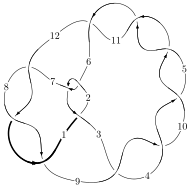
\includegraphics[width=112pt]{../../../GIT/diagram.site/Diagrams/png/1377_12a_0576.png}\\
\ \ \ A knot diagram\footnotemark}&
\allowdisplaybreaks
\textbf{Linearized knot diagam} \\
\cline{2-2}
 &
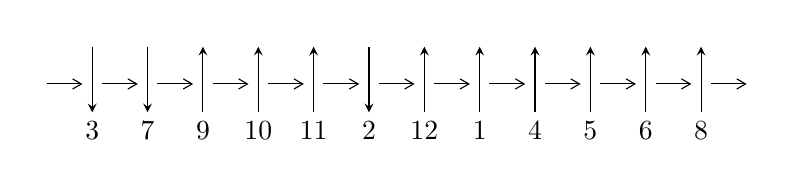
\begin{tikzpicture}[x=20pt, y=17pt]
	% nodes
	\node (C0) at (0, 0) {};
	\node (C1) at (1, 0) {};
	\node (C1U) at (1, +1) {};
	\node (C1D) at (1, -1) {3};

	\node (C2) at (2, 0) {};
	\node (C2U) at (2, +1) {};
	\node (C2D) at (2, -1) {7};

	\node (C3) at (3, 0) {};
	\node (C3U) at (3, +1) {};
	\node (C3D) at (3, -1) {9};

	\node (C4) at (4, 0) {};
	\node (C4U) at (4, +1) {};
	\node (C4D) at (4, -1) {10};

	\node (C5) at (5, 0) {};
	\node (C5U) at (5, +1) {};
	\node (C5D) at (5, -1) {11};

	\node (C6) at (6, 0) {};
	\node (C6U) at (6, +1) {};
	\node (C6D) at (6, -1) {2};

	\node (C7) at (7, 0) {};
	\node (C7U) at (7, +1) {};
	\node (C7D) at (7, -1) {12};

	\node (C8) at (8, 0) {};
	\node (C8U) at (8, +1) {};
	\node (C8D) at (8, -1) {1};

	\node (C9) at (9, 0) {};
	\node (C9U) at (9, +1) {};
	\node (C9D) at (9, -1) {4};

	\node (C10) at (10, 0) {};
	\node (C10U) at (10, +1) {};
	\node (C10D) at (10, -1) {5};

	\node (C11) at (11, 0) {};
	\node (C11U) at (11, +1) {};
	\node (C11D) at (11, -1) {6};

	\node (C12) at (12, 0) {};
	\node (C12U) at (12, +1) {};
	\node (C12D) at (12, -1) {8};
	\node (C13) at (13, 0) {};

	% arrows
	\draw[->,>={angle 60}]
	(C0) edge (C1) (C1) edge (C2) (C2) edge (C3) (C3) edge (C4) (C4) edge (C5) (C5) edge (C6) (C6) edge (C7) (C7) edge (C8) (C8) edge (C9) (C9) edge (C10) (C10) edge (C11) (C11) edge (C12) (C12) edge (C13) ;	\draw[->,>=stealth]
	(C1U) edge (C1D) (C2U) edge (C2D) (C3D) edge (C3U) (C4D) edge (C4U) (C5D) edge (C5U) (C6U) edge (C6D) (C7D) edge (C7U) (C8D) edge (C8U) (C9D) edge (C9U) (C10D) edge (C10U) (C11D) edge (C11U) (C12D) edge (C12U) ;
	\end{tikzpicture} \\
\hhline{~~} \\& 
\textbf{Solving Sequence} \\ \cline{2-2} 
 &
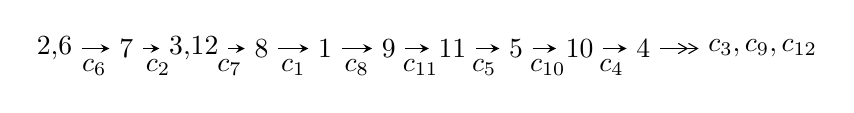
\begin{tikzpicture}[x=23pt, y=7pt]
	% node
	\node (A0) at (-1/8, 0) {2,6};
	\node (A1) at (1, 0) {7};
	\node (A2) at (33/16, 0) {3,12};
	\node (A3) at (25/8, 0) {8};
	\node (A4) at (33/8, 0) {1};
	\node (A5) at (41/8, 0) {9};
	\node (A6) at (49/8, 0) {11};
	\node (A7) at (57/8, 0) {5};
	\node (A8) at (65/8, 0) {10};
	\node (A9) at (73/8, 0) {4};
	\node (C1) at (1/2, -1) {$c_{6}$};
	\node (C2) at (3/2, -1) {$c_{2}$};
	\node (C3) at (21/8, -1) {$c_{7}$};
	\node (C4) at (29/8, -1) {$c_{1}$};
	\node (C5) at (37/8, -1) {$c_{8}$};
	\node (C6) at (45/8, -1) {$c_{11}$};
	\node (C7) at (53/8, -1) {$c_{5}$};
	\node (C8) at (61/8, -1) {$c_{10}$};
	\node (C9) at (69/8, -1) {$c_{4}$};
	\node (A10) at (11, 0) {$c_{3},c_{9},c_{12}$};

	% edge
	\draw[->,>=stealth]	
	(A0) edge (A1) (A1) edge (A2) (A2) edge (A3) (A3) edge (A4) (A4) edge (A5) (A5) edge (A6) (A6) edge (A7) (A7) edge (A8) (A8) edge (A9) ;
	\draw[->>,>={angle 60}]	
	(A9) edge (A10);
\end{tikzpicture} \\ 

\end{tabular} \\

\footnotetext{
The image of knot diagram is generated by the software ``\textbf{Draw programme}" developed by Andrew Bartholomew(\url{http://www.layer8.co.uk/maths/draw/index.htm\#Running-draw}), where we modified some parts for our purpose(\url{https://github.com/CATsTAILs/LinksPainter}).
}\phantom \\ \newline 
\centering \textbf{Ideals for irreducible components\footnotemark of $X_{\text{par}}$} 
 
\begin{align*}
I^u_{1}&=\langle 
11985 u^{24}+25005 u^{23}+\cdots+72188 b-244730,\\
\phantom{I^u_{1}}&\phantom{= \langle  }-211795 u^{24}-38567 u^{23}+\cdots+505316 a-3814672,\;u^{25}- u^{24}+\cdots-9 u-7\rangle \\
I^u_{2}&=\langle 
u^3+b- u,\;a+u,\;u^9-3 u^7+u^6+3 u^5-2 u^4-3 u^3+u^2+2 u-1\rangle \\
I^u_{3}&=\langle 
b- a+1,\;a^2-2 a-2,\;u+1\rangle \\
I^u_{4}&=\langle 
b-1,\;a,\;u-1\rangle \\
I^u_{5}&=\langle 
b+1,\;a+2,\;u-1\rangle \\
I^u_{6}&=\langle 
b-1,\;a-1,\;u-1\rangle \\
I^u_{7}&=\langle 
b,\;a-1,\;u+1\rangle \\
\\
I^v_{1}&=\langle 
a,\;b+1,\;v+1\rangle \\
\end{align*}
\raggedright * 8 irreducible components of $\dim_{\mathbb{C}}=0$, with total 41 representations.\\
\footnotetext{All coefficients of polynomials are rational numbers. But the coefficients are sometimes approximated in decimal forms when there is not enough margin.}
\newpage
\renewcommand{\arraystretch}{1}
\centering \section*{I. $I^u_{1}= \langle 11985 u^{24}+25005 u^{23}+\cdots+72188 b-244730,\;-2.12\times10^{5} u^{24}-3.86\times10^{4} u^{23}+\cdots+5.05\times10^{5} a-3.81\times10^{6},\;u^{25}- u^{24}+\cdots-9 u-7 \rangle$}
\flushleft \textbf{(i) Arc colorings}\\
\begin{tabular}{m{7pt} m{180pt} m{7pt} m{180pt} }
\flushright $a_{2}=$&$\begin{pmatrix}0\\u\end{pmatrix}$ \\
\flushright $a_{6}=$&$\begin{pmatrix}1\\0\end{pmatrix}$ \\
\flushright $a_{7}=$&$\begin{pmatrix}1\\u^2\end{pmatrix}$ \\
\flushright $a_{3}=$&$\begin{pmatrix}- u\\- u^3+u\end{pmatrix}$ \\
\flushright $a_{12}=$&$\begin{pmatrix}0.419134 u^{24}+0.0763225 u^{23}+\cdots-0.423143 u+7.54908\\-0.166025 u^{24}-0.346387 u^{23}+\cdots+2.60629 u+3.39018\end{pmatrix}$ \\
\flushright $a_{8}=$&$\begin{pmatrix}0.484311 u^{24}-0.650336 u^{23}+\cdots+12.6564 u-0.752505\\-0.101956 u^{24}-0.126046 u^{23}+\cdots+0.520322 u-3.17143\end{pmatrix}$ \\
\flushright $a_{1}=$&$\begin{pmatrix}u^3\\u^5- u^3+u\end{pmatrix}$ \\
\flushright $a_{9}=$&$\begin{pmatrix}-0.523558 u^{24}-0.576639 u^{23}+\cdots+3.23109 u-5.84862\\0.409514 u^{24}+0.597509 u^{23}+\cdots-4.14134 u-3.60527\end{pmatrix}$ \\
\flushright $a_{11}=$&$\begin{pmatrix}0.585159 u^{24}+0.422710 u^{23}+\cdots-3.02944 u+4.15891\\-0.166025 u^{24}-0.346387 u^{23}+\cdots+2.60629 u+3.39018\end{pmatrix}$ \\
\flushright $a_{5}=$&$\begin{pmatrix}-0.995781 u^{24}-0.0732195 u^{23}+\cdots-7.99477 u+3.18634\\0.246842 u^{24}+0.673949 u^{23}+\cdots-7.09679 u+2.13396\end{pmatrix}$ \\
\flushright $a_{10}=$&$\begin{pmatrix}-0.479844 u^{24}-0.692303 u^{23}+\cdots+4.66701 u-9.17722\\0.348285 u^{24}+0.294232 u^{23}+\cdots-0.412423 u-4.84612\end{pmatrix}$ \\
\flushright $a_{4}=$&$\begin{pmatrix}1.37385 u^{24}-0.126816 u^{23}+\cdots+11.2503 u-2.86998\\0.198759 u^{24}-1.06936 u^{23}+\cdots+15.0646 u+1.75878\end{pmatrix}$\\&\end{tabular}
\flushleft \textbf{(ii) Obstruction class $= -1$}\\~\\
\flushleft \textbf{(iii) Cusp Shapes $= -\frac{60407}{36094} u^{24}+\frac{67585}{36094} u^{23}+\cdots-\frac{588579}{36094} u+\frac{309390}{18047}$}\\~\\
\newpage\renewcommand{\arraystretch}{1}
\flushleft \textbf{(iv) u-Polynomials at the component}\newline \\
\begin{tabular}{m{50pt}|m{274pt}}
Crossings & \hspace{64pt}u-Polynomials at each crossing \\
\hline $$\begin{aligned}c_{1}\end{aligned}$$&$\begin{aligned}
&u^{25}+7 u^{24}+\cdots+739 u+49
\end{aligned}$\\
\hline $$\begin{aligned}c_{2},c_{6}\end{aligned}$$&$\begin{aligned}
&u^{25}- u^{24}+\cdots-9 u-7
\end{aligned}$\\
\hline $$\begin{aligned}c_{3},c_{4},c_{5}\\c_{9},c_{10},c_{11}\end{aligned}$$&$\begin{aligned}
&u^{25}+2 u^{24}+\cdots+2 u+2
\end{aligned}$\\
\hline $$\begin{aligned}c_{7},c_{8},c_{12}\end{aligned}$$&$\begin{aligned}
&u^{25}+u^{24}+\cdots+39 u-9
\end{aligned}$\\
\hline
\end{tabular}\\~\\
\newpage\renewcommand{\arraystretch}{1}
\flushleft \textbf{(v) Riley Polynomials at the component}\newline \\
\begin{tabular}{m{50pt}|m{274pt}}
Crossings & \hspace{64pt}Riley Polynomials at each crossing \\
\hline $$\begin{aligned}c_{1}\end{aligned}$$&$\begin{aligned}
&y^{25}+29 y^{24}+\cdots+138539 y-2401
\end{aligned}$\\
\hline $$\begin{aligned}c_{2},c_{6}\end{aligned}$$&$\begin{aligned}
&y^{25}-7 y^{24}+\cdots+739 y-49
\end{aligned}$\\
\hline $$\begin{aligned}c_{3},c_{4},c_{5}\\c_{9},c_{10},c_{11}\end{aligned}$$&$\begin{aligned}
&y^{25}-36 y^{24}+\cdots+147 y^2-4
\end{aligned}$\\
\hline $$\begin{aligned}c_{7},c_{8},c_{12}\end{aligned}$$&$\begin{aligned}
&y^{25}-31 y^{24}+\cdots+1755 y-81
\end{aligned}$\\
\hline
\end{tabular}\\~\\
\newpage\flushleft \textbf{(vi) Complex Volumes and Cusp Shapes}
$$\begin{array}{c|c|c}  
\text{Solutions to }I^u_{1}& \I (\text{vol} + \sqrt{-1}CS) & \text{Cusp shape}\\
 \hline 
\begin{aligned}
u &= \phantom{-}0.896141 + 0.476708 I \\
a &= \phantom{-}0.264009 + 1.247940 I \\
b &= -0.518330 + 0.326163 I\end{aligned}
 & -0.17909 - 3.47166 I & \phantom{-}8.30266 + 8.94170 I \\ \hline\begin{aligned}
u &= \phantom{-}0.896141 - 0.476708 I \\
a &= \phantom{-}0.264009 - 1.247940 I \\
b &= -0.518330 - 0.326163 I\end{aligned}
 & -0.17909 + 3.47166 I & \phantom{-}8.30266 - 8.94170 I \\ \hline\begin{aligned}
u &= \phantom{-}0.712580 + 0.800068 I \\
a &= -0.424664 - 0.601315 I \\
b &= -0.730693 - 0.421612 I\end{aligned}
 & \phantom{-}6.89461 + 0.59668 I & \phantom{-}14.2492 - 1.6095 I \\ \hline\begin{aligned}
u &= \phantom{-}0.712580 - 0.800068 I \\
a &= -0.424664 + 0.601315 I \\
b &= -0.730693 + 0.421612 I\end{aligned}
 & \phantom{-}6.89461 - 0.59668 I & \phantom{-}14.2492 + 1.6095 I \\ \hline\begin{aligned}
u &= -0.871015 + 0.279677 I \\
a &= -0.337858 + 0.872649 I \\
b &= -0.111064 + 0.372277 I\end{aligned}
 & -1.37494 + 1.08288 I & \phantom{-}0.78629 - 1.57388 I \\ \hline\begin{aligned}
u &= -0.871015 - 0.279677 I \\
a &= -0.337858 - 0.872649 I \\
b &= -0.111064 - 0.372277 I\end{aligned}
 & -1.37494 - 1.08288 I & \phantom{-}0.78629 + 1.57388 I \\ \hline\begin{aligned}
u &= -1.09658\phantom{ +0.000000I} \\
a &= -1.64444\phantom{ +0.000000I} \\
b &= -1.74239\phantom{ +0.000000I}\end{aligned}
 & \phantom{-}11.6378\phantom{ +0.000000I} & \phantom{-}5.99100\phantom{ +0.000000I} \\ \hline\begin{aligned}
u &= -0.874419 + 0.729333 I \\
a &= \phantom{-}0.344893 - 1.149310 I \\
b &= \phantom{-}0.073544 - 0.603993 I\end{aligned}
 & \phantom{-}4.42212 + 2.78000 I & \phantom{-}9.55915 - 2.23614 I \\ \hline\begin{aligned}
u &= -0.874419 - 0.729333 I \\
a &= \phantom{-}0.344893 + 1.149310 I \\
b &= \phantom{-}0.073544 + 0.603993 I\end{aligned}
 & \phantom{-}4.42212 - 2.78000 I & \phantom{-}9.55915 + 2.23614 I \\ \hline\begin{aligned}
u &= -0.582867 + 0.979338 I \\
a &= \phantom{-}0.091026 - 0.120602 I \\
b &= \phantom{-}1.354550 - 0.178353 I\end{aligned}
 & \phantom{-}13.77140 - 2.72282 I & \phantom{-}16.3024 + 1.1923 I\\
 \hline 
 \end{array}$$\newpage$$\begin{array}{c|c|c}  
\text{Solutions to }I^u_{1}& \I (\text{vol} + \sqrt{-1}CS) & \text{Cusp shape}\\
 \hline 
\begin{aligned}
u &= -0.582867 - 0.979338 I \\
a &= \phantom{-}0.091026 + 0.120602 I \\
b &= \phantom{-}1.354550 + 0.178353 I\end{aligned}
 & \phantom{-}13.77140 + 2.72282 I & \phantom{-}16.3024 - 1.1923 I \\ \hline\begin{aligned}
u &= -0.947893 + 0.650696 I \\
a &= -0.21022 + 1.47307 I \\
b &= \phantom{-}1.250280 + 0.142199 I\end{aligned}
 & \phantom{-}5.58852 + 5.07025 I & \phantom{-}11.97391 - 5.86575 I \\ \hline\begin{aligned}
u &= -0.947893 - 0.650696 I \\
a &= -0.21022 - 1.47307 I \\
b &= \phantom{-}1.250280 - 0.142199 I\end{aligned}
 & \phantom{-}5.58852 - 5.07025 I & \phantom{-}11.97391 + 5.86575 I \\ \hline\begin{aligned}
u &= \phantom{-}0.544687 + 1.115460 I \\
a &= \phantom{-}0.171496 + 0.032811 I \\
b &= -1.82545 - 0.04307 I\end{aligned}
 & -13.8936 + 3.7790 I & \phantom{-}16.4732 - 0.8824 I \\ \hline\begin{aligned}
u &= \phantom{-}0.544687 - 1.115460 I \\
a &= \phantom{-}0.171496 - 0.032811 I \\
b &= -1.82545 + 0.04307 I\end{aligned}
 & -13.8936 - 3.7790 I & \phantom{-}16.4732 + 0.8824 I \\ \hline\begin{aligned}
u &= \phantom{-}1.006720 + 0.738523 I \\
a &= -0.027411 - 1.413620 I \\
b &= \phantom{-}0.601135 - 0.505413 I\end{aligned}
 & \phantom{-}6.00828 - 6.40238 I & \phantom{-}12.19839 + 6.95987 I \\ \hline\begin{aligned}
u &= \phantom{-}1.006720 - 0.738523 I \\
a &= -0.027411 + 1.413620 I \\
b &= \phantom{-}0.601135 + 0.505413 I\end{aligned}
 & \phantom{-}6.00828 + 6.40238 I & \phantom{-}12.19839 - 6.95987 I \\ \hline\begin{aligned}
u &= \phantom{-}1.000710 + 0.748113 I \\
a &= \phantom{-}0.18239 + 1.58644 I \\
b &= -1.80123 + 0.03491 I\end{aligned}
 & \phantom{-}16.8362 - 5.8723 I & \phantom{-}12.48696 + 4.57611 I \\ \hline\begin{aligned}
u &= \phantom{-}1.000710 - 0.748113 I \\
a &= \phantom{-}0.18239 - 1.58644 I \\
b &= -1.80123 - 0.03491 I\end{aligned}
 & \phantom{-}16.8362 + 5.8723 I & \phantom{-}12.48696 - 4.57611 I \\ \hline\begin{aligned}
u &= -1.124230 + 0.767226 I \\
a &= -0.28369 - 1.52440 I \\
b &= -1.290050 - 0.256043 I\end{aligned}
 & \phantom{-}12.1250 + 9.0916 I & \phantom{-}14.3993 - 5.8572 I\\
 \hline 
 \end{array}$$\newpage$$\begin{array}{c|c|c}  
\text{Solutions to }I^u_{1}& \I (\text{vol} + \sqrt{-1}CS) & \text{Cusp shape}\\
 \hline 
\begin{aligned}
u &= -1.124230 - 0.767226 I \\
a &= -0.28369 + 1.52440 I \\
b &= -1.290050 + 0.256043 I\end{aligned}
 & \phantom{-}12.1250 - 9.0916 I & \phantom{-}14.3993 + 5.8572 I \\ \hline\begin{aligned}
u &= \phantom{-}1.20486 + 0.78616 I \\
a &= \phantom{-}0.47352 - 1.57215 I \\
b &= \phantom{-}1.81036 - 0.06682 I\end{aligned}
 & -15.9680 - 10.6007 I & \phantom{-}14.6369 + 4.9142 I \\ \hline\begin{aligned}
u &= \phantom{-}1.20486 - 0.78616 I \\
a &= \phantom{-}0.47352 + 1.57215 I \\
b &= \phantom{-}1.81036 + 0.06682 I\end{aligned}
 & -15.9680 + 10.6007 I & \phantom{-}14.6369 - 4.9142 I \\ \hline\begin{aligned}
u &= \phantom{-}0.539518\phantom{ +0.000000I} \\
a &= -0.734615\phantom{ +0.000000I} \\
b &= \phantom{-}0.400542\phantom{ +0.000000I}\end{aligned}
 & \phantom{-}0.694972\phantom{ +0.000000I} & \phantom{-}14.9110\phantom{ +0.000000I} \\ \hline\begin{aligned}
u &= -0.373488\phantom{ +0.000000I} \\
a &= \phantom{-}4.17778\phantom{ +0.000000I} \\
b &= \phantom{-}1.71576\phantom{ +0.000000I}\end{aligned}
 & \phantom{-}14.6126\phantom{ +0.000000I} & \phantom{-}18.3610\phantom{ +0.000000I}\\
 \hline 
 \end{array}$$\newpage\newpage\renewcommand{\arraystretch}{1}
\centering \section*{II. $I^u_{2}= \langle u^3+b- u,\;a+u,\;u^9-3 u^7+u^6+3 u^5-2 u^4-3 u^3+u^2+2 u-1 \rangle$}
\flushleft \textbf{(i) Arc colorings}\\
\begin{tabular}{m{7pt} m{180pt} m{7pt} m{180pt} }
\flushright $a_{2}=$&$\begin{pmatrix}0\\u\end{pmatrix}$ \\
\flushright $a_{6}=$&$\begin{pmatrix}1\\0\end{pmatrix}$ \\
\flushright $a_{7}=$&$\begin{pmatrix}1\\u^2\end{pmatrix}$ \\
\flushright $a_{3}=$&$\begin{pmatrix}- u\\- u^3+u\end{pmatrix}$ \\
\flushright $a_{12}=$&$\begin{pmatrix}- u\\- u^3+u\end{pmatrix}$ \\
\flushright $a_{8}=$&$\begin{pmatrix}u^2+1\\u^4\end{pmatrix}$ \\
\flushright $a_{1}=$&$\begin{pmatrix}u^3\\u^5- u^3+u\end{pmatrix}$ \\
\flushright $a_{9}=$&$\begin{pmatrix}- u^4+u^2+1\\- u^6+2 u^4- u^2\end{pmatrix}$ \\
\flushright $a_{11}=$&$\begin{pmatrix}u^3-2 u\\- u^3+u\end{pmatrix}$ \\
\flushright $a_{5}=$&$\begin{pmatrix}- u^6+3 u^4-2 u^2+1\\u^6-2 u^4+u^2\end{pmatrix}$ \\
\flushright $a_{10}=$&$\begin{pmatrix}u^7+u^6-2 u^5-2 u^4+u^3+u^2- u-1\\- u^6+2 u^4+u^3- u^2- u+1\end{pmatrix}$ \\
\flushright $a_{4}=$&$\begin{pmatrix}u^7-2 u^5\\- u^6+2 u^4+u^3- u^2- u+1\end{pmatrix}$\\&\end{tabular}
\flushleft \textbf{(ii) Obstruction class $= -1$}\\~\\
\flushleft \textbf{(iii) Cusp Shapes $= 14$}\\~\\
\newpage\renewcommand{\arraystretch}{1}
\flushleft \textbf{(iv) u-Polynomials at the component}\newline \\
\begin{tabular}{m{50pt}|m{274pt}}
Crossings & \hspace{64pt}u-Polynomials at each crossing \\
\hline $$\begin{aligned}c_{1}\end{aligned}$$&$\begin{aligned}
&u^9+6 u^8+15 u^7+25 u^6+35 u^5+36 u^4+27 u^3+17 u^2+6 u+1
\end{aligned}$\\
\hline $$\begin{aligned}c_{2},c_{6},c_{7}\\c_{8},c_{12}\end{aligned}$$&$\begin{aligned}
&u^9-3 u^7+u^6+3 u^5-2 u^4-3 u^3+u^2+2 u-1
\end{aligned}$\\
\hline $$\begin{aligned}c_{3},c_{4},c_{5}\\c_{9},c_{10},c_{11}\end{aligned}$$&$\begin{aligned}
&(u^3- u^2-2 u+1)^3
\end{aligned}$\\
\hline
\end{tabular}\\~\\
\newpage\renewcommand{\arraystretch}{1}
\flushleft \textbf{(v) Riley Polynomials at the component}\newline \\
\begin{tabular}{m{50pt}|m{274pt}}
Crossings & \hspace{64pt}Riley Polynomials at each crossing \\
\hline $$\begin{aligned}c_{1}\end{aligned}$$&$\begin{aligned}
&y^9-6 y^8-5 y^7+47 y^6+43 y^5-88 y^4-125 y^3-37 y^2+2 y-1
\end{aligned}$\\
\hline $$\begin{aligned}c_{2},c_{6},c_{7}\\c_{8},c_{12}\end{aligned}$$&$\begin{aligned}
&y^9-6 y^8+15 y^7-25 y^6+35 y^5-36 y^4+27 y^3-17 y^2+6 y-1
\end{aligned}$\\
\hline $$\begin{aligned}c_{3},c_{4},c_{5}\\c_{9},c_{10},c_{11}\end{aligned}$$&$\begin{aligned}
&(y^3-5 y^2+6 y-1)^3
\end{aligned}$\\
\hline
\end{tabular}\\~\\
\newpage\flushleft \textbf{(vi) Complex Volumes and Cusp Shapes}
$$\begin{array}{c|c|c}  
\text{Solutions to }I^u_{2}& \I (\text{vol} + \sqrt{-1}CS) & \text{Cusp shape}\\
 \hline 
\begin{aligned}
u &= -0.689884 + 0.654080 I \\
a &= \phantom{-}0.689884 - 0.654080 I \\
b &= -1.24698\phantom{ +0.000000I}\end{aligned}
 & \phantom{-}6.34475\phantom{ +0.000000I} & \phantom{-}14.0000\phantom{ +0.000000I} \\ \hline\begin{aligned}
u &= -0.689884 - 0.654080 I \\
a &= \phantom{-}0.689884 + 0.654080 I \\
b &= -1.24698\phantom{ +0.000000I}\end{aligned}
 & \phantom{-}6.34475\phantom{ +0.000000I} & \phantom{-}14.0000\phantom{ +0.000000I} \\ \hline\begin{aligned}
u &= \phantom{-}0.743582 + 0.811631 I \\
a &= -0.743582 - 0.811631 I \\
b &= \phantom{-}1.80194\phantom{ +0.000000I}\end{aligned}
 & \phantom{-}17.6243\phantom{ +0.000000I} & \phantom{-}14.0000\phantom{ +0.000000I} \\ \hline\begin{aligned}
u &= \phantom{-}0.743582 - 0.811631 I \\
a &= -0.743582 + 0.811631 I \\
b &= \phantom{-}1.80194\phantom{ +0.000000I}\end{aligned}
 & \phantom{-}17.6243\phantom{ +0.000000I} & \phantom{-}14.0000\phantom{ +0.000000I} \\ \hline\begin{aligned}
u &= -1.17430\phantom{ +0.000000I} \\
a &= \phantom{-}1.17430\phantom{ +0.000000I} \\
b &= \phantom{-}0.445042\phantom{ +0.000000I}\end{aligned}
 & \phantom{-}0.704972\phantom{ +0.000000I} & \phantom{-}14.0000\phantom{ +0.000000I} \\ \hline\begin{aligned}
u &= \phantom{-}1.37977\phantom{ +0.000000I} \\
a &= -1.37977\phantom{ +0.000000I} \\
b &= -1.24698\phantom{ +0.000000I}\end{aligned}
 & \phantom{-}6.34475\phantom{ +0.000000I} & \phantom{-}14.0000\phantom{ +0.000000I} \\ \hline\begin{aligned}
u &= \phantom{-}0.587151 + 0.185036 I \\
a &= -0.587151 - 0.185036 I \\
b &= \phantom{-}0.445042\phantom{ +0.000000I}\end{aligned}
 & \phantom{-}0.704972\phantom{ +0.000000I} & \phantom{-}14.0000\phantom{ +0.000000I} \\ \hline\begin{aligned}
u &= \phantom{-}0.587151 - 0.185036 I \\
a &= -0.587151 + 0.185036 I \\
b &= \phantom{-}0.445042\phantom{ +0.000000I}\end{aligned}
 & \phantom{-}0.704972\phantom{ +0.000000I} & \phantom{-}14.0000\phantom{ +0.000000I} \\ \hline\begin{aligned}
u &= -1.48716\phantom{ +0.000000I} \\
a &= \phantom{-}1.48716\phantom{ +0.000000I} \\
b &= \phantom{-}1.80194\phantom{ +0.000000I}\end{aligned}
 & \phantom{-}17.6243\phantom{ +0.000000I} & \phantom{-}14.0000\phantom{ +0.000000I}\\
 \hline 
 \end{array}$$\newpage\newpage\renewcommand{\arraystretch}{1}
\centering \section*{III. $I^u_{3}= \langle b- a+1,\;a^2-2 a-2,\;u+1 \rangle$}
\flushleft \textbf{(i) Arc colorings}\\
\begin{tabular}{m{7pt} m{180pt} m{7pt} m{180pt} }
\flushright $a_{2}=$&$\begin{pmatrix}0\\-1\end{pmatrix}$ \\
\flushright $a_{6}=$&$\begin{pmatrix}1\\0\end{pmatrix}$ \\
\flushright $a_{7}=$&$\begin{pmatrix}1\\1\end{pmatrix}$ \\
\flushright $a_{3}=$&$\begin{pmatrix}1\\0\end{pmatrix}$ \\
\flushright $a_{12}=$&$\begin{pmatrix}a\\a-1\end{pmatrix}$ \\
\flushright $a_{8}=$&$\begin{pmatrix}a+1\\a\end{pmatrix}$ \\
\flushright $a_{1}=$&$\begin{pmatrix}-1\\-1\end{pmatrix}$ \\
\flushright $a_{9}=$&$\begin{pmatrix}a\\a-1\end{pmatrix}$ \\
\flushright $a_{11}=$&$\begin{pmatrix}1\\a-1\end{pmatrix}$ \\
\flushright $a_{5}=$&$\begin{pmatrix}a\\3\end{pmatrix}$ \\
\flushright $a_{10}=$&$\begin{pmatrix}- a-1\\-2 a+2\end{pmatrix}$ \\
\flushright $a_{4}=$&$\begin{pmatrix}- a-1\\-3\end{pmatrix}$\\&\end{tabular}
\flushleft \textbf{(ii) Obstruction class $= 1$}\\~\\
\flushleft \textbf{(iii) Cusp Shapes $= 12$}\\~\\
\newpage\renewcommand{\arraystretch}{1}
\flushleft \textbf{(iv) u-Polynomials at the component}\newline \\
\begin{tabular}{m{50pt}|m{274pt}}
Crossings & \hspace{64pt}u-Polynomials at each crossing \\
\hline $$\begin{aligned}c_{1},c_{2},c_{12}\end{aligned}$$&$\begin{aligned}
&(u-1)^2
\end{aligned}$\\
\hline $$\begin{aligned}c_{3},c_{4},c_{5}\\c_{9},c_{10},c_{11}\end{aligned}$$&$\begin{aligned}
&u^2-3
\end{aligned}$\\
\hline $$\begin{aligned}c_{6},c_{7},c_{8}\end{aligned}$$&$\begin{aligned}
&(u+1)^2
\end{aligned}$\\
\hline
\end{tabular}\\~\\
\newpage\renewcommand{\arraystretch}{1}
\flushleft \textbf{(v) Riley Polynomials at the component}\newline \\
\begin{tabular}{m{50pt}|m{274pt}}
Crossings & \hspace{64pt}Riley Polynomials at each crossing \\
\hline $$\begin{aligned}c_{1},c_{2},c_{6}\\c_{7},c_{8},c_{12}\end{aligned}$$&$\begin{aligned}
&(y-1)^2
\end{aligned}$\\
\hline $$\begin{aligned}c_{3},c_{4},c_{5}\\c_{9},c_{10},c_{11}\end{aligned}$$&$\begin{aligned}
&(y-3)^2
\end{aligned}$\\
\hline
\end{tabular}\\~\\
\newpage\flushleft \textbf{(vi) Complex Volumes and Cusp Shapes}
$$\begin{array}{c|c|c}  
\text{Solutions to }I^u_{3}& \I (\text{vol} + \sqrt{-1}CS) & \text{Cusp shape}\\
 \hline 
\begin{aligned}
u &= -1.00000\phantom{ +0.000000I} \\
a &= -0.732051\phantom{ +0.000000I} \\
b &= -1.73205\phantom{ +0.000000I}\end{aligned}
 & \phantom{-}13.1595\phantom{ +0.000000I} & \phantom{-}12.0000\phantom{ +0.000000I} \\ \hline\begin{aligned}
u &= -1.00000\phantom{ +0.000000I} \\
a &= \phantom{-}2.73205\phantom{ +0.000000I} \\
b &= \phantom{-}1.73205\phantom{ +0.000000I}\end{aligned}
 & \phantom{-}13.1595\phantom{ +0.000000I} & \phantom{-}12.0000\phantom{ +0.000000I}\\
 \hline 
 \end{array}$$\newpage\newpage\renewcommand{\arraystretch}{1}
\centering \section*{IV. $I^u_{4}= \langle b-1,\;a,\;u-1 \rangle$}
\flushleft \textbf{(i) Arc colorings}\\
\begin{tabular}{m{7pt} m{180pt} m{7pt} m{180pt} }
\flushright $a_{2}=$&$\begin{pmatrix}0\\1\end{pmatrix}$ \\
\flushright $a_{6}=$&$\begin{pmatrix}1\\0\end{pmatrix}$ \\
\flushright $a_{7}=$&$\begin{pmatrix}1\\1\end{pmatrix}$ \\
\flushright $a_{3}=$&$\begin{pmatrix}-1\\0\end{pmatrix}$ \\
\flushright $a_{12}=$&$\begin{pmatrix}0\\1\end{pmatrix}$ \\
\flushright $a_{8}=$&$\begin{pmatrix}1\\0\end{pmatrix}$ \\
\flushright $a_{1}=$&$\begin{pmatrix}1\\1\end{pmatrix}$ \\
\flushright $a_{9}=$&$\begin{pmatrix}0\\-1\end{pmatrix}$ \\
\flushright $a_{11}=$&$\begin{pmatrix}-1\\1\end{pmatrix}$ \\
\flushright $a_{5}=$&$\begin{pmatrix}0\\1\end{pmatrix}$ \\
\flushright $a_{10}=$&$\begin{pmatrix}-1\\0\end{pmatrix}$ \\
\flushright $a_{4}=$&$\begin{pmatrix}-1\\1\end{pmatrix}$\\&\end{tabular}
\flushleft \textbf{(ii) Obstruction class $= 1$}\\~\\
\flushleft \textbf{(iii) Cusp Shapes $= 12$}\\~\\
\newpage\renewcommand{\arraystretch}{1}
\flushleft \textbf{(iv) u-Polynomials at the component}\newline \\
\begin{tabular}{m{50pt}|m{274pt}}
Crossings & \hspace{64pt}u-Polynomials at each crossing \\
\hline $$\begin{aligned}c_{1},c_{3},c_{4}\\c_{5},c_{6},c_{7}\\c_{8}\end{aligned}$$&$\begin{aligned}
&u-1
\end{aligned}$\\
\hline $$\begin{aligned}c_{2},c_{9},c_{10}\\c_{11},c_{12}\end{aligned}$$&$\begin{aligned}
&u+1
\end{aligned}$\\
\hline
\end{tabular}\\~\\
\newpage\renewcommand{\arraystretch}{1}
\flushleft \textbf{(v) Riley Polynomials at the component}\newline \\
\begin{tabular}{m{50pt}|m{274pt}}
Crossings & \hspace{64pt}Riley Polynomials at each crossing \\
\hline $$\begin{aligned}c_{1},c_{2},c_{3}\\c_{4},c_{5},c_{6}\\c_{7},c_{8},c_{9}\\c_{10},c_{11},c_{12}\end{aligned}$$&$\begin{aligned}
&y-1
\end{aligned}$\\
\hline
\end{tabular}\\~\\
\newpage\flushleft \textbf{(vi) Complex Volumes and Cusp Shapes}
$$\begin{array}{c|c|c}  
\text{Solutions to }I^u_{4}& \I (\text{vol} + \sqrt{-1}CS) & \text{Cusp shape}\\
 \hline 
\begin{aligned}
u &= \phantom{-}1.00000\phantom{ +0.000000I} \\
a &= \phantom{-0.000000 } 0 \\
b &= \phantom{-}1.00000\phantom{ +0.000000I}\end{aligned}
 & \phantom{-}3.28987\phantom{ +0.000000I} & \phantom{-}12.0000\phantom{ +0.000000I}\\
 \hline 
 \end{array}$$\newpage\newpage\renewcommand{\arraystretch}{1}
\centering \section*{V. $I^u_{5}= \langle b+1,\;a+2,\;u-1 \rangle$}
\flushleft \textbf{(i) Arc colorings}\\
\begin{tabular}{m{7pt} m{180pt} m{7pt} m{180pt} }
\flushright $a_{2}=$&$\begin{pmatrix}0\\1\end{pmatrix}$ \\
\flushright $a_{6}=$&$\begin{pmatrix}1\\0\end{pmatrix}$ \\
\flushright $a_{7}=$&$\begin{pmatrix}1\\1\end{pmatrix}$ \\
\flushright $a_{3}=$&$\begin{pmatrix}-1\\0\end{pmatrix}$ \\
\flushright $a_{12}=$&$\begin{pmatrix}-2\\-1\end{pmatrix}$ \\
\flushright $a_{8}=$&$\begin{pmatrix}3\\2\end{pmatrix}$ \\
\flushright $a_{1}=$&$\begin{pmatrix}1\\1\end{pmatrix}$ \\
\flushright $a_{9}=$&$\begin{pmatrix}2\\1\end{pmatrix}$ \\
\flushright $a_{11}=$&$\begin{pmatrix}-1\\-1\end{pmatrix}$ \\
\flushright $a_{5}=$&$\begin{pmatrix}2\\1\end{pmatrix}$ \\
\flushright $a_{10}=$&$\begin{pmatrix}1\\0\end{pmatrix}$ \\
\flushright $a_{4}=$&$\begin{pmatrix}1\\1\end{pmatrix}$\\&\end{tabular}
\flushleft \textbf{(ii) Obstruction class $= 1$}\\~\\
\flushleft \textbf{(iii) Cusp Shapes $= 12$}\\~\\
\newpage\renewcommand{\arraystretch}{1}
\flushleft \textbf{(iv) u-Polynomials at the component}\newline \\
\begin{tabular}{m{50pt}|m{274pt}}
Crossings & \hspace{64pt}u-Polynomials at each crossing \\
\hline $$\begin{aligned}c_{1},c_{6},c_{7}\\c_{8},c_{9},c_{10}\\c_{11}\end{aligned}$$&$\begin{aligned}
&u-1
\end{aligned}$\\
\hline $$\begin{aligned}c_{2},c_{3},c_{4}\\c_{5},c_{12}\end{aligned}$$&$\begin{aligned}
&u+1
\end{aligned}$\\
\hline
\end{tabular}\\~\\
\newpage\renewcommand{\arraystretch}{1}
\flushleft \textbf{(v) Riley Polynomials at the component}\newline \\
\begin{tabular}{m{50pt}|m{274pt}}
Crossings & \hspace{64pt}Riley Polynomials at each crossing \\
\hline $$\begin{aligned}c_{1},c_{2},c_{3}\\c_{4},c_{5},c_{6}\\c_{7},c_{8},c_{9}\\c_{10},c_{11},c_{12}\end{aligned}$$&$\begin{aligned}
&y-1
\end{aligned}$\\
\hline
\end{tabular}\\~\\
\newpage\flushleft \textbf{(vi) Complex Volumes and Cusp Shapes}
$$\begin{array}{c|c|c}  
\text{Solutions to }I^u_{5}& \I (\text{vol} + \sqrt{-1}CS) & \text{Cusp shape}\\
 \hline 
\begin{aligned}
u &= \phantom{-}1.00000\phantom{ +0.000000I} \\
a &= -2.00000\phantom{ +0.000000I} \\
b &= -1.00000\phantom{ +0.000000I}\end{aligned}
 & \phantom{-}3.28987\phantom{ +0.000000I} & \phantom{-}12.0000\phantom{ +0.000000I}\\
 \hline 
 \end{array}$$\newpage\newpage\renewcommand{\arraystretch}{1}
\centering \section*{VI. $I^u_{6}= \langle b-1,\;a-1,\;u-1 \rangle$}
\flushleft \textbf{(i) Arc colorings}\\
\begin{tabular}{m{7pt} m{180pt} m{7pt} m{180pt} }
\flushright $a_{2}=$&$\begin{pmatrix}0\\1\end{pmatrix}$ \\
\flushright $a_{6}=$&$\begin{pmatrix}1\\0\end{pmatrix}$ \\
\flushright $a_{7}=$&$\begin{pmatrix}1\\1\end{pmatrix}$ \\
\flushright $a_{3}=$&$\begin{pmatrix}-1\\0\end{pmatrix}$ \\
\flushright $a_{12}=$&$\begin{pmatrix}1\\1\end{pmatrix}$ \\
\flushright $a_{8}=$&$\begin{pmatrix}1\\1\end{pmatrix}$ \\
\flushright $a_{1}=$&$\begin{pmatrix}1\\1\end{pmatrix}$ \\
\flushright $a_{9}=$&$\begin{pmatrix}1\\1\end{pmatrix}$ \\
\flushright $a_{11}=$&$\begin{pmatrix}0\\1\end{pmatrix}$ \\
\flushright $a_{5}=$&$\begin{pmatrix}1\\1\end{pmatrix}$ \\
\flushright $a_{10}=$&$\begin{pmatrix}-1\\0\end{pmatrix}$ \\
\flushright $a_{4}=$&$\begin{pmatrix}0\\1\end{pmatrix}$\\&\end{tabular}
\flushleft \textbf{(ii) Obstruction class $= -1$}\\~\\
\flushleft \textbf{(iii) Cusp Shapes $= 6$}\\~\\
\newpage\renewcommand{\arraystretch}{1}
\flushleft \textbf{(iv) u-Polynomials at the component}\newline \\
\begin{tabular}{m{50pt}|m{274pt}}
Crossings & \hspace{64pt}u-Polynomials at each crossing \\
\hline $$\begin{aligned}c_{1}\end{aligned}$$&$\begin{aligned}
&u+1
\end{aligned}$\\
\hline $$\begin{aligned}c_{2},c_{3},c_{4}\\c_{5},c_{6},c_{9}\\c_{10},c_{11}\end{aligned}$$&$\begin{aligned}
&u-1
\end{aligned}$\\
\hline $$\begin{aligned}c_{7},c_{8},c_{12}\end{aligned}$$&$\begin{aligned}
&u
\end{aligned}$\\
\hline
\end{tabular}\\~\\
\newpage\renewcommand{\arraystretch}{1}
\flushleft \textbf{(v) Riley Polynomials at the component}\newline \\
\begin{tabular}{m{50pt}|m{274pt}}
Crossings & \hspace{64pt}Riley Polynomials at each crossing \\
\hline $$\begin{aligned}c_{1},c_{2},c_{3}\\c_{4},c_{5},c_{6}\\c_{9},c_{10},c_{11}\end{aligned}$$&$\begin{aligned}
&y-1
\end{aligned}$\\
\hline $$\begin{aligned}c_{7},c_{8},c_{12}\end{aligned}$$&$\begin{aligned}
&y
\end{aligned}$\\
\hline
\end{tabular}\\~\\
\newpage\flushleft \textbf{(vi) Complex Volumes and Cusp Shapes}
$$\begin{array}{c|c|c}  
\text{Solutions to }I^u_{6}& \I (\text{vol} + \sqrt{-1}CS) & \text{Cusp shape}\\
 \hline 
\begin{aligned}
u &= \phantom{-}1.00000\phantom{ +0.000000I} \\
a &= \phantom{-}1.00000\phantom{ +0.000000I} \\
b &= \phantom{-}1.00000\phantom{ +0.000000I}\end{aligned}
 & \phantom{-}1.64493\phantom{ +0.000000I} & \phantom{-}6.00000\phantom{ +0.000000I}\\
 \hline 
 \end{array}$$\newpage\newpage\renewcommand{\arraystretch}{1}
\centering \section*{VII. $I^u_{7}= \langle b,\;a-1,\;u+1 \rangle$}
\flushleft \textbf{(i) Arc colorings}\\
\begin{tabular}{m{7pt} m{180pt} m{7pt} m{180pt} }
\flushright $a_{2}=$&$\begin{pmatrix}0\\-1\end{pmatrix}$ \\
\flushright $a_{6}=$&$\begin{pmatrix}1\\0\end{pmatrix}$ \\
\flushright $a_{7}=$&$\begin{pmatrix}1\\1\end{pmatrix}$ \\
\flushright $a_{3}=$&$\begin{pmatrix}1\\0\end{pmatrix}$ \\
\flushright $a_{12}=$&$\begin{pmatrix}1\\0\end{pmatrix}$ \\
\flushright $a_{8}=$&$\begin{pmatrix}2\\1\end{pmatrix}$ \\
\flushright $a_{1}=$&$\begin{pmatrix}-1\\-1\end{pmatrix}$ \\
\flushright $a_{9}=$&$\begin{pmatrix}1\\0\end{pmatrix}$ \\
\flushright $a_{11}=$&$\begin{pmatrix}1\\0\end{pmatrix}$ \\
\flushright $a_{5}=$&$\begin{pmatrix}1\\0\end{pmatrix}$ \\
\flushright $a_{10}=$&$\begin{pmatrix}1\\0\end{pmatrix}$ \\
\flushright $a_{4}=$&$\begin{pmatrix}1\\0\end{pmatrix}$\\&\end{tabular}
\flushleft \textbf{(ii) Obstruction class $= 1$}\\~\\
\flushleft \textbf{(iii) Cusp Shapes $= 0$}\\~\\
\newpage\renewcommand{\arraystretch}{1}
\flushleft \textbf{(iv) u-Polynomials at the component}\newline \\
\begin{tabular}{m{50pt}|m{274pt}}
Crossings & \hspace{64pt}u-Polynomials at each crossing \\
\hline $$\begin{aligned}c_{1},c_{2},c_{12}\end{aligned}$$&$\begin{aligned}
&u-1
\end{aligned}$\\
\hline $$\begin{aligned}c_{3},c_{4},c_{5}\\c_{9},c_{10},c_{11}\end{aligned}$$&$\begin{aligned}
&u
\end{aligned}$\\
\hline $$\begin{aligned}c_{6},c_{7},c_{8}\end{aligned}$$&$\begin{aligned}
&u+1
\end{aligned}$\\
\hline
\end{tabular}\\~\\
\newpage\renewcommand{\arraystretch}{1}
\flushleft \textbf{(v) Riley Polynomials at the component}\newline \\
\begin{tabular}{m{50pt}|m{274pt}}
Crossings & \hspace{64pt}Riley Polynomials at each crossing \\
\hline $$\begin{aligned}c_{1},c_{2},c_{6}\\c_{7},c_{8},c_{12}\end{aligned}$$&$\begin{aligned}
&y-1
\end{aligned}$\\
\hline $$\begin{aligned}c_{3},c_{4},c_{5}\\c_{9},c_{10},c_{11}\end{aligned}$$&$\begin{aligned}
&y
\end{aligned}$\\
\hline
\end{tabular}\\~\\
\newpage\flushleft \textbf{(vi) Complex Volumes and Cusp Shapes}
$$\begin{array}{c|c|c}  
\text{Solutions to }I^u_{7}& \I (\text{vol} + \sqrt{-1}CS) & \text{Cusp shape}\\
 \hline 
\begin{aligned}
u &= -1.00000\phantom{ +0.000000I} \\
a &= \phantom{-}1.00000\phantom{ +0.000000I} \\
b &= \phantom{-0.000000 } 0\end{aligned}
 & \phantom{-0.000000 } 0 & \phantom{-0.000000 } 0\\
 \hline 
 \end{array}$$\newpage\newpage\renewcommand{\arraystretch}{1}
\centering \section*{VIII. $I^v_{1}= \langle a,\;b+1,\;v+1 \rangle$}
\flushleft \textbf{(i) Arc colorings}\\
\begin{tabular}{m{7pt} m{180pt} m{7pt} m{180pt} }
\flushright $a_{2}=$&$\begin{pmatrix}-1\\0\end{pmatrix}$ \\
\flushright $a_{6}=$&$\begin{pmatrix}1\\0\end{pmatrix}$ \\
\flushright $a_{7}=$&$\begin{pmatrix}1\\0\end{pmatrix}$ \\
\flushright $a_{3}=$&$\begin{pmatrix}-1\\0\end{pmatrix}$ \\
\flushright $a_{12}=$&$\begin{pmatrix}0\\-1\end{pmatrix}$ \\
\flushright $a_{8}=$&$\begin{pmatrix}1\\-1\end{pmatrix}$ \\
\flushright $a_{1}=$&$\begin{pmatrix}-1\\0\end{pmatrix}$ \\
\flushright $a_{9}=$&$\begin{pmatrix}0\\-1\end{pmatrix}$ \\
\flushright $a_{11}=$&$\begin{pmatrix}1\\-1\end{pmatrix}$ \\
\flushright $a_{5}=$&$\begin{pmatrix}0\\1\end{pmatrix}$ \\
\flushright $a_{10}=$&$\begin{pmatrix}1\\0\end{pmatrix}$ \\
\flushright $a_{4}=$&$\begin{pmatrix}-1\\1\end{pmatrix}$\\&\end{tabular}
\flushleft \textbf{(ii) Obstruction class $= -1$}\\~\\
\flushleft \textbf{(iii) Cusp Shapes $= 18$}\\~\\
\newpage\renewcommand{\arraystretch}{1}
\flushleft \textbf{(iv) u-Polynomials at the component}\newline \\
\begin{tabular}{m{50pt}|m{274pt}}
Crossings & \hspace{64pt}u-Polynomials at each crossing \\
\hline $$\begin{aligned}c_{1},c_{2},c_{6}\end{aligned}$$&$\begin{aligned}
&u
\end{aligned}$\\
\hline $$\begin{aligned}c_{3},c_{4},c_{5}\\c_{7},c_{8},c_{9}\\c_{10},c_{11},c_{12}\end{aligned}$$&$\begin{aligned}
&u+1
\end{aligned}$\\
\hline
\end{tabular}\\~\\
\newpage\renewcommand{\arraystretch}{1}
\flushleft \textbf{(v) Riley Polynomials at the component}\newline \\
\begin{tabular}{m{50pt}|m{274pt}}
Crossings & \hspace{64pt}Riley Polynomials at each crossing \\
\hline $$\begin{aligned}c_{1},c_{2},c_{6}\end{aligned}$$&$\begin{aligned}
&y
\end{aligned}$\\
\hline $$\begin{aligned}c_{3},c_{4},c_{5}\\c_{7},c_{8},c_{9}\\c_{10},c_{11},c_{12}\end{aligned}$$&$\begin{aligned}
&y-1
\end{aligned}$\\
\hline
\end{tabular}\\~\\
\newpage\flushleft \textbf{(vi) Complex Volumes and Cusp Shapes}
$$\begin{array}{c|c|c}  
\text{Solutions to }I^v_{1}& \I (\text{vol} + \sqrt{-1}CS) & \text{Cusp shape}\\
 \hline 
\begin{aligned}
v &= -1.00000\phantom{ +0.000000I} \\
a &= \phantom{-0.000000 } 0 \\
b &= -1.00000\phantom{ +0.000000I}\end{aligned}
 & \phantom{-}4.93480\phantom{ +0.000000I} & \phantom{-}18.0000\phantom{ +0.000000I}\\
 \hline 
 \end{array}$$\newpage
\newpage\renewcommand{\arraystretch}{1}
\centering \section*{ IX. u-Polynomials}
\begin{tabular}{m{50pt}|m{274pt}}
Crossings & \hspace{64pt}u-Polynomials at each crossing \\
\hline $$\begin{aligned}c_{1}\end{aligned}$$&$\begin{aligned}
&u(u-1)^5(u+1)\\
&\cdot(u^9+6 u^8+15 u^7+25 u^6+35 u^5+36 u^4+27 u^3+17 u^2+6 u+1)\\
&\cdot(u^{25}+7 u^{24}+\cdots+739 u+49)
\end{aligned}$\\
\hline $$\begin{aligned}c_{2}\end{aligned}$$&$\begin{aligned}
&u(u-1)^4(u+1)^2(u^9-3 u^7+u^6+3 u^5-2 u^4-3 u^3+u^2+2 u-1)\\
&\cdot(u^{25}- u^{24}+\cdots-9 u-7)
\end{aligned}$\\
\hline $$\begin{aligned}c_{3},c_{4},c_{5}\\c_{9},c_{10},c_{11}\end{aligned}$$&$\begin{aligned}
&u(u-1)^2(u+1)^2(u^2-3)(u^3- u^2-2 u+1)^3\\
&\cdot(u^{25}+2 u^{24}+\cdots+2 u+2)
\end{aligned}$\\
\hline $$\begin{aligned}c_{6}\end{aligned}$$&$\begin{aligned}
&u(u-1)^3(u+1)^3(u^9-3 u^7+u^6+3 u^5-2 u^4-3 u^3+u^2+2 u-1)\\
&\cdot(u^{25}- u^{24}+\cdots-9 u-7)
\end{aligned}$\\
\hline $$\begin{aligned}c_{7},c_{8}\end{aligned}$$&$\begin{aligned}
&u(u-1)^2(u+1)^4(u^9-3 u^7+u^6+3 u^5-2 u^4-3 u^3+u^2+2 u-1)\\
&\cdot(u^{25}+u^{24}+\cdots+39 u-9)
\end{aligned}$\\
\hline $$\begin{aligned}c_{12}\end{aligned}$$&$\begin{aligned}
&u(u-1)^3(u+1)^3(u^9-3 u^7+u^6+3 u^5-2 u^4-3 u^3+u^2+2 u-1)\\
&\cdot(u^{25}+u^{24}+\cdots+39 u-9)
\end{aligned}$\\
\hline
\end{tabular}\newpage\renewcommand{\arraystretch}{1}
\centering \section*{ X. Riley Polynomials}
\begin{tabular}{m{50pt}|m{274pt}}
Crossings & \hspace{64pt}Riley Polynomials at each crossing \\
\hline $$\begin{aligned}c_{1}\end{aligned}$$&$\begin{aligned}
&y(y-1)^6\\
&\cdot(y^9-6 y^8-5 y^7+47 y^6+43 y^5-88 y^4-125 y^3-37 y^2+2 y-1)\\
&\cdot(y^{25}+29 y^{24}+\cdots+138539 y-2401)
\end{aligned}$\\
\hline $$\begin{aligned}c_{2},c_{6}\end{aligned}$$&$\begin{aligned}
&y(y-1)^6\\
&\cdot(y^9-6 y^8+15 y^7-25 y^6+35 y^5-36 y^4+27 y^3-17 y^2+6 y-1)\\
&\cdot(y^{25}-7 y^{24}+\cdots+739 y-49)
\end{aligned}$\\
\hline $$\begin{aligned}c_{3},c_{4},c_{5}\\c_{9},c_{10},c_{11}\end{aligned}$$&$\begin{aligned}
&y(y-3)^2(y-1)^4(y^3-5 y^2+6 y-1)^3\\
&\cdot(y^{25}-36 y^{24}+\cdots+147 y^2-4)
\end{aligned}$\\
\hline $$\begin{aligned}c_{7},c_{8},c_{12}\end{aligned}$$&$\begin{aligned}
&y(y-1)^6\\
&\cdot(y^9-6 y^8+15 y^7-25 y^6+35 y^5-36 y^4+27 y^3-17 y^2+6 y-1)\\
&\cdot(y^{25}-31 y^{24}+\cdots+1755 y-81)
\end{aligned}$\\
\hline
\end{tabular}
\vskip 2pc
\end{document}